%%%%%%%%%%%%%%%%%%%%%%%%%%%%%%%%%%%%%
% Document properties and packages
%%%%%%%%%%%%%%%%%%%%%%%%%%%%%%%%%%%%%
\documentclass[a4paper,12pt,final]{memoir}
% \usepackage{CJKutf8}%中文支持
\usepackage[UTF8]{ctex}
% \usepackage{xeCJK}
\usepackage{float}
% misc
\renewcommand{\familydefault}{bch}	% font
\pagestyle{empty}					% no pagenumbering
\setlength{\parindent}{0pt}			% no paragraph indentation
% required packages (add your own)
\usepackage{flowfram}% column layou
\usepackage{marvosym}
\usepackage{textcomp}

\usepackage[top=1cm,left=1cm,right=1cm,bottom=1cm]{geometry}% margins
\usepackage{graphicx}										% figures
\usepackage{hyperref}
\definecolor{linkcolour}{rgb}{0,0.2,0.6}  %蓝色
\hypersetup{colorlinks,breaklinks,urlcolor=linkcolour, linkcolor=linkcolour}										% URLs
\usepackage[usenames,dvipsnames]{xcolor}					% color
\usepackage{multicol}										% columns env.
	\setlength{\multicolsep}{0pt}
\usepackage{paralist}										% compact lists
\usepackage{tikz}

%%%%%%%%%%%%%%%%%%%%%%%%%%%%%%%%%%%%%
% Create column layout
%%%%%%%%%%%%%%%%%%%%%%%%%%%%%%%%%%%%%
% define length commands
\setlength{\vcolumnsep}{\baselineskip}
\setlength{\columnsep}{\vcolumnsep}
%定义主题颜色,可选颜色 Maroon,ForestGreen,DarkOrchid,RoyalBlue,Turquoise,Cyan,etc,更多颜色参考xcolor包的颜色定义
\newcommand{\myThemeColor}{RoyalBlue}
% frame setup (flowfram package)
% left frame
\newflowframe{0.23\textwidth}{\textheight}{0pt}{0pt}[left]
	\newlength{\LeftMainSep}
	\setlength{\LeftMainSep}{0.23\textwidth}
	\addtolength{\LeftMainSep}{1\columnsep}
 
% small static frame for the vertical line
\newstaticframe{1.5pt}{\textheight}{\LeftMainSep}{0pt}
 
% content of the static frame
\begin{staticcontents}{1} %绘制分割线,使用tikz包绘制。如需改变风格线样式,请参考tikz教程,对于新手,不建议修改。
\hfill
\tikz{%
	\draw[loosely dotted,color=\myThemeColor,line width=1.5pt,yshift=0]
	(0,0) -- (0,\textheight);}%
\hfill\mbox{}
\end{staticcontents}
 
% right frame
\addtolength{\LeftMainSep}{1.5pt}
\addtolength{\LeftMainSep}{1\columnsep}
\newflowframe{0.7\textwidth}{\textheight}{\LeftMainSep}{0pt}[main01]


%%%%%%%%%%%%%%%%%%%%%%%%%%%%%%%%%%%%%
% define macros (for convience)
%%%%%%%%%%%%%%%%%%%%%%%%%%%%%%%%%%%%%
\newcommand{\Sep}{\vspace{1em}}
\newcommand{\SmallSep}{\vspace{0.9em}}

\newenvironment{AboutMe}
	{\ignorespaces\textbf{\color{\myThemeColor} About me}}
	{\Sep\ignorespacesafterend}
%定义section	
\newcommand{\CVSection}[1]
	{\Large\textbf{#1}\par
	\vspace{0.2cm}\normalsize\normalfont}

\newcommand{\CVItem}[1]
	{\textbf{\color{\myThemeColor} #1}}


%%%%%%%%%%%%%%%%%%%%%%%%%%%%%%%%%%%%%
% Begin document
%%%%%%%%%%%%%%%%%%%%%%%%%%%%%%%%%%%%%
\begin{document}

% \begin{CJK*}{UTF8}{gbsn}%选择字体,黑体
% Left frame 左边内容在此定义
%%%%%%%%%%%%%%%%%%%%
\begin{figure}
	\hfill
	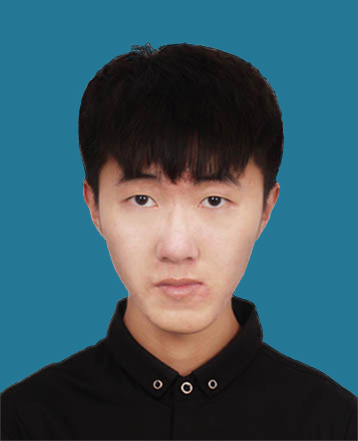
\includegraphics[width=0.8\columnwidth]{../img/photo.jpg}
	\vspace{-7cm}
\end{figure}
\begin{flushright}\footnotesize
.\\
\vskip 6cm
    \raggedright
	\CVItem{{\large 个人信息:}}\\
	Email:\\
	\href{mailto:jiafeng5513@outlook.com}{jiafeng5513@outlook.com}  \\
	Github:\\
	\href{github.com/jiafeng5513}{github.com/jiafeng5513} \\
	Tel:\\
	15764356880
	\SmallSep
	\SmallSep

	\CVItem{{\large 技能:}}\\
	$\bullet$\textbf{编程语言:}\\ C\#/C++/Java/Python\\
	$\bullet$\textbf{专长:}\\ 深度学习/模型部署/高性能计算/多平台客户端开发 \\
	% \SmallSep
	% \textit{具备较丰富的桌面客户端,机器视觉和深度学习的开发经验,对U3D和UE4具有一定的使用经验,有较强的学习能力,具备英文文献查阅理解和写作能力.}

	\SmallSep
	\SmallSep
	\SmallSep
	
	\CVItem{\large Link To My Github}
	\begin{figure}[h]
		\centering
		
\includegraphics[width=0.8\columnwidth]{../img/Github.png}
	\end{figure}
	

\end{flushright}\normalsize
\framebreak


% Right frame 右边内容在此定义
%%%%%%%%%%%%%%%%%%%%
\Huge\bfseries {\color{\myThemeColor} 贾~~锋}\\
\normalsize\normalfont

% Education
\CVSection{主要经历}
\hrule
\SmallSep

\CVItem{2022.07 - 现在\hfill\textsc{英特尔亚太研发有限公司}}\\
\textit{-Intel's Software and Advanced Technology Group (SATG)}\\
\textit{-高性能计算工程师}

\CVItem{2020.07 - 2022.07\hfill\textsc{华为技术有限公司}}\\
\textit{-智能驾驶解决方案BU}\\
\textit{-高性能计算工程师}

\CVItem{2013.09 - 2020.07\hfill\textsc{吉林大学}}\\
\textit{-计算机科学与技术学院}\\
\textit{-计算机图形学方向,硕士学位}
\\

% CAMPU
\CVSection{工作内容}
\hrule
\SmallSep
\CVItem{LLM 部署\hfill\emph{英特尔}}\\
\textit{$\bullet$ 在英特尔平台上支持大模型(DeepSeek-R1、QWen3、MiniCPM)部署。使用的软件平台为oneAPI-IPEX-torch 和 oneAPI-OpenVINO, 硬件平台为英特尔x86架构的CPU,以及NPU、核显和Arc系列独立显卡. }

\CVItem{LLM训练以及应用开发\hfill\emph{英特尔}}\\
\textit{$\bullet$ 
开发了数个基于LLM和VLM的应用,例如为AIPC开发的Windows应用和为智能座舱开发的安卓应用。这些应用在2025年上海车展、2023年金博会和2025年CES上展出。与面壁智能(ModelBest)合作,训练了GUI Agent模型并开发了相关应用,该应用可以根据语音指令直接帮助用户操作安卓设备的图形界面。} 
\\
\CVItem{算子开发\hfill\emph{华为}}\\
\textit{$\bullet$ 
在华为ADS平台上开发深度学习算子和机器视觉算子。使用的软件平台为华为的Mindspore,硬件平台为基于ARM架构的昇腾610和615芯片。其中CPU算子使用ARM SVE指令集,主要实现一些机器视觉算法,NPU算子使用类汇编的Intrinsics,主要支持模型推理。两年期间交付约30个算子。}
\\
\CVItem{CI/CD \hfill\emph{华为}}\\
\textit{$\bullet$ 
为ADS软件平台设计并实现了AI模型的CI/CD系统,将模型转换和算子嵌入过程集成到CI/CD流程,实现从训练代码和数据集到最终的端侧模型的版本跟踪,帮助算子开发满足华为ICSL规范。}
\\

% HONORS & SCHOLARSHIPS
\CVSection{获奖}
\hrule
\SmallSep
	\begin{tabular}{l|l}
		$\Rightarrow$ 英特尔&\textit{ 2024年,年度员工。}\footnotesize\\
		$\Rightarrow$ 华为&\textit{ 2022年,华为明日之星。}\\
	\end{tabular}

%%%%%%%%%%%%%%%%%%%%%%%%%%%%%%%%%%%%%
% End document
%%%%%%%%%%%%%%%%%%%%%%%%%%%%%%%%%%%%%
% \end{CJK*}
\end{document}